\documentclass[12pt,article]{article}
\usepackage{fullpage}
\usepackage[top=2cm, bottom=4.5cm, left=2cm, right=2cm]{geometry}
\usepackage{amsmath,amsthm,amsfonts,amssymb,amscd}
\usepackage{lastpage}
\usepackage{enumerate}
\usepackage{fancyhdr}
\usepackage{mathrsfs}
\usepackage{xcolor}
\usepackage{graphicx}
\usepackage{listings}
\usepackage{hyperref}
\usepackage{mdframed}
\usepackage{changepage}   % for the adjustwidth environment
\usepackage{forest} 
\usepackage{tikz}   % For graph

\usepackage{float}  % To inforce inserting images at the right place
\restylefloat{table}

\usepackage[center]{caption}

\usepackage{caption}
\usepackage{subcaption}

\usepackage{algorithm}
\usepackage{algpseudocode}
\usepackage{graphicx,txfonts}


% For recursive formulation, adapted from https://tex.stackexchange.com/questions/580333/typing-sequences-recursively-in-overleaf
\usepackage{mathtools}
\makeatletter
\newcases{centercases}{\quad}
  {\hfil$\m@th\displaystyle{##}$\hfil}
  {$\m@th\displaystyle{##}$\hfil}{\lbrace}{.}
\makeatother

\newcommand{\Tau}{\mathrm{T}}
\newcommand{\heart}{\ensuremath\varheartsuit}


% For matrix
\def\horzbar{\text{magic}}

\hypersetup{%
  colorlinks=true,
  linkcolor=blue,
  linkbordercolor={0 0 1}
}

\setlength{\parindent}{0.0in}
\setlength{\parskip}{0.05in}

\newcommand\projnumber{4}
\newcommand\course{CS534}
\newcommand\OSUID{934370552}
\newcommand\Email{buivy@oregonstate.edu}
\newcommand\Name{Vy Bui}
\newcommand\tab[1][1cm]{\hspace*{#1}}

\pagestyle{fancyplain}
\headheight 35pt
\lhead{Homework \projnumber}
\rhead{Mar 8, 2023}
\lfoot{}
\cfoot{}
\rfoot{\small\thepage}
\headsep 1.5em

\newenvironment{task}[2][Task]
    { \begin{mdframed}[backgroundcolor=gray!20] \textbf{#1 #2} \\}
    {  \end{mdframed}}
   

% Make Rightarrow with superscript
% \makeatletter
% \newcommand{\xRightarrow}[2][]{\ext@arrow 0359\Rightarrowfill@{#1}{#2}}
% \makeatother

\begin{document}

\begin{titlepage}
    \begin{center}
        \vspace*{4cm}

        \textbf{\Large AI539 - Natural Language Processing with Deep Learning}

        \vspace{0.5cm}
 
        \textbf{ Homework \projnumber \ Report}

        \textbf{ Attention Mechanisms in Sequence-to-Sequence Models }
 
        \vspace{1cm}

        Author: Vy Bui

        OSUID: 934370552

        \vspace{1cm}

        Instructor: Professor Stefan Lee
        \vfill
             
        \vspace{0.8cm}
      
             
        The School of Electrical Engineering and Computer Science\\
        Oregon State University\\
             
    \end{center}
\end{titlepage}


%==============================================================================%
%

\begin{task}{1.1} 
\textbf{Copying} [2pts]

Describe (in one or two sentences) what properties of the keys and queries would result in the output $\mathbf{a}$ being equal to one of the input values $\mathbf{v}_j$. Specifically, what must be true about the query $\mathbf{q}$ and the keys $\mathbf{k}_1, ..., \mathbf{k}_m$ such that $\mathbf{a} \approx \mathbf{v}_j$? (We assume all values are unique -- $\mathbf{v}_i \neq \mathbf{v}_j,~\forall ij$.)
\end{task}

The keys and the query must be orthogonal to have zero dot products, except for the dot product 
$$<q,k_i> = <x_i,x_i>$$

This makes all $\alpha$ approach zero except for $\alpha_j$ being close to 1.
%==============================================================================%
\begin{task}{1.2} 
\textbf{Average of Two} [2pts]

Consider a set of key vectors $\{\mathbf{k}_1, ... , \mathbf{k}_m\}$ where all keys are orthogonal unit vectors -- that is to say $\mathbf{k}_i\mathbf{k}_j^T =0,~\forall ij$ and $||\mathbf{k}_i||=1,~\forall i$. Let $\mathbf{v}_a, \mathbf{v}_b \in \{\mathbf{v}_1, ..., \mathbf{v}_m\}$ be two value vectors. Give an expression for a query vector $\mathbf{q}$ such that the output $\mathbf{a}$ is approximately equal to the average of $\mathbf{v}_a$ and $\mathbf{v}_b$, that is to say $\mathbf{a} \approx \frac{1}{2}(\mathbf{v}_a + \mathbf{v}_b)$. You can reference the key vectors corresponding to $\mathbf{v}_a$ and $\mathbf{v}_b$ as $\mathbf{k}_a$ and $\mathbf{k_b}$ respectively. Note that due to the softmax in Eq. 1, it won't ever actually reach this value, but you can make it arbitrarily close by adding a scaling constant to your solution.
\end{task}

q should have all entries equal zero except for two entries $q_a = q_b = t$ corresponding to $v_a$ and $v_b$ respectively. This will result in following proportional scores

\begin{eqnarray}
\alpha_a = \frac{\mbox{exp}\left(~\mathbf{q}\mathbf{k}_a^T / \sqrt d\right)}{\sum_{j=1}^m \mbox{exp}\left(\mathbf{q}\mathbf{k}_j^T / \sqrt d\right)} = \frac{\mbox{exp}\left(~\mathbf{q}\mathbf{k}_a^T / \sqrt d\right)}{1 + 1 + ... + \mbox{exp}\left(\mathbf{q}\mathbf{k}_a^T / \sqrt d\right) + \mbox{exp}\left(\mathbf{q}\mathbf{k}_b^T / \sqrt d\right)} 
= \frac{\mbox{exp}\left(t / \sqrt d\right)}{m - 2 + 2 \mbox{exp}\left(t / \sqrt d\right)} = \alpha_b
\end{eqnarray}

\begin{eqnarray}
\alpha_i = \frac{1}{m - 2 + 2 \mbox{exp}\left(t / \sqrt d\right)}, i \neq a,b
\end{eqnarray}

$\alpha_a$ and $\alpha_b$ will approach $\frac{1}{2}$ when t becomes larger.

%==============================================================================%
\newpage
\begin{task}{1.3} 
\textbf{Noisy Average} [2pts]

Now consider a set of key vectors $\{\mathbf{k}_1, ... , \mathbf{k}_m\}$ where keys are randomly scaled such that $\mathbf{k}_i = \mathbf{\mu}_i*\lambda_i$ where $\lambda_i \sim \mathcal{N}(1, \beta)$ is a randomly sampled scalar multiplier. Assume the unscaled vectors $\mu_1, ..., \mu_m$ are orthogonal unit vectors. If you use the same strategy to construct the query $q$ as you did in Task 1.2, what would be the outcome here? Specifically, derive $\mathbf{q}\mathbf{k}_a^T$ and $\mathbf{q}\mathbf{k}_b^T$ in terms of $\mu$'s and $\lambda$'s. Qualitatively describe what how the output $a$ would vary over multiple resamplings of $\lambda_1, ..., \lambda_m$.
\end{task}
Using the same $q$ from task 1.2 results in the following dot products
$$qk_a^T = t \mu_a \lambda_a = t \lambda_a$$
$$qk_b^T = t \mu_b \lambda_b = t \lambda_b$$

and propotional scores 
\begin{eqnarray}
\alpha_a = \frac{\mbox{exp}\left(t \lambda_a / \sqrt d\right)}{m - 2 + \mbox{exp}\left(t \lambda_a / \sqrt d\right) + \mbox{exp}\left(t \lambda_b / \sqrt d\right)}
\end{eqnarray}

\begin{eqnarray}
\alpha_b = \frac{\mbox{exp}\left(t \lambda_b / \sqrt d\right)}{m - 2 + \mbox{exp}\left(t \lambda_a / \sqrt d\right) + \mbox{exp}\left(t \lambda_b / \sqrt d\right)}
\end{eqnarray}

Sampling $\lambda$ k times from $\mathcal{N}(1,\beta)$ results in a sample with mean $E[\overline{\lambda}] = 1$ and $Var(\overline{\lambda}) = \beta/k$. As a result, vector $a$ is expected to be $\frac{v_a + v_b}{2}$, but can also be skewed towards either $v_a$ or $v_b$.
%==============================================================================%
\begin{task}{1.4} 
\textbf{Noisy Average with Multi-head Attention} [2pts]

Let's now consider a simple version of multi-head attention that averages the attended features resulting from two different queries. Here, two queries are defined ($\mathbf{q}_1$ and $\mathbf{q}_2$) leading to two different attended features ($\mathbf{a}_1$ and $\mathbf{a}_2$). The output of this computation will be $\mathbf{a} = \frac{1}{2}(\mathbf{a}_1 + \mathbf{a}_2)$. Assume we have keys like those in Task 1.3, design queries $\mathbf{q}_1$ and $\mathbf{q}_2$ such that $\mathbf{a} \approx \frac{1}{2}(\mathbf{v}_a + \mathbf{v}_b)$.
\end{task}

%==============================================================================%
\newpage
\begin{task}{2.1} 
\textbf{Scaled-Dot Product Attention} [8pts]

Implement $\mbox{Attn}(\cdot)$ in equation (11) as single-query scaled dot-product attention as defined in equations (1) and (2). Here, the query will be the decoder hidden state and the keys and values will be derived from the encoder representations. Implement this attention mechanism by completing the \texttt{SingleQueryScaledDotProductAttention} class in \texttt{mt\_driver.py}.

%
\noindent The forward function takes two inputs -- \texttt{hidden} is the decoder hidden state $h_j^{(d)}$ and \texttt{encoder\_outputs} corresponds to encoder word representations $h_t^{(e)},~\forall t$. These should be converted to keys, queries, and values:
\begin{eqnarray}
\mathbf{q} = W_q \mathbf{h}_j^{(d)}\\
\mathbf{k}_t = W_k \mathbf{h}_t^{(e)}\\
\mathbf{v}_t = \mathbf{h}_t^{(e)}
\end{eqnarray}
\noindent And the output -- \texttt{attended\_val} and \texttt{alpha} -- correspond to the attended value vector ($\mathbf{a}$) and the vector of attention values ($\alpha$) computed from as in equations (1) and (2). The expected dimensions are asserted above. Note that this is intended to be a batched operation and the equations presented are for a single instance. \texttt{torch.bmm} can be very useful here.\\[8pt]

\noindent Train this model by executing  \texttt{python mt\_driver.py}. Record the perplexity and BLEU score on the test set. These are automatically generated in the script and printed after training.
\end{task}

The model produced a test loss of 1.854, perplexity of 6.384, and BLEU of 33.76.

%==============================================================================%
\newpage
\begin{task}{2.2} 
\textbf{Attention Diagrams} [1pts]

Search through the attention diagrams produced by your model. Include a few examples in your report and characterize common patterns you observe.Note that German is (mostly) a Subject-Object-Verb language so you may find attention patterns that indicate inversion of word order when translating to Subject-Verb-Object English as in the 2nd example above.
\end{task}

\begin{figure}[H]
    \centering
    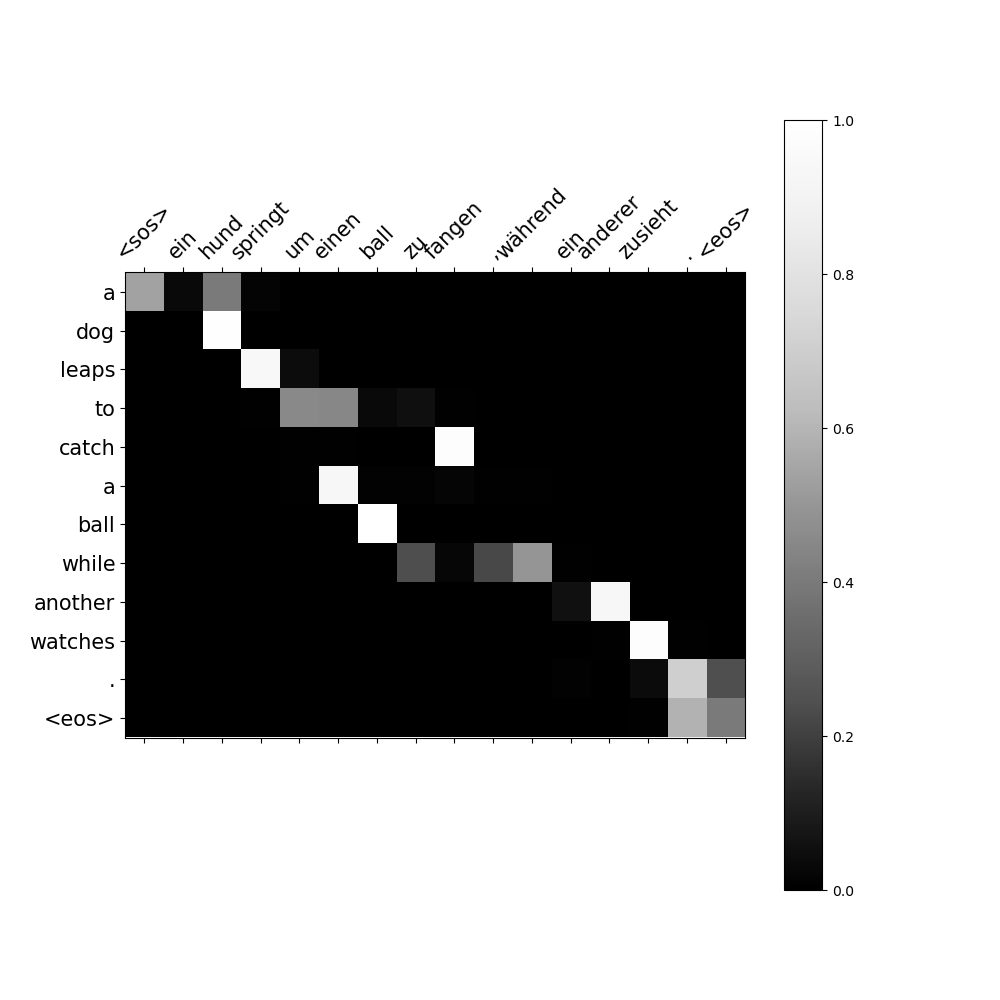
\includegraphics[scale=0.5]{281_translation.png} \par
    \caption{A translation example}
    \label{fig:trans-ex}
\end{figure}

Figure \ref{fig:trans-ex} shows the inversion of word order in English-German translation. In particular, the verb "fangen" follows object "ball" in German, where as the verb "catch" precedes object "ball" in English.

%==============================================================================%
\newpage
\begin{task}{2.3} 
\textbf{Comparison} [3pts]

Train and evaluate models with the \texttt{Dummy} and \texttt{MeanPool} `attention' mechanisms. Report mean and variance over three runs for these baselines and your implementation of scaled dot-product attention. Discuss the observed trends.
\end{task}

\begin{center}
    \begin{tabular}{ |c|c|c|c|c| } 
    \hline
    & PPL mean & PPL variance & BLEU mean & BLEU variance \\
    \hline
    dummy & 10.874 & 0.012 & 19.107 & 0.005 \\
    \hline
    mean & 9.021 & 0.005 & 23.22 & 0.082 \\
    \hline
    sdp & 6.421 & 0.007 & 34.413 & 0.429 \\
    \hline
    \end{tabular}
    
    Table 1: comparison of different attention mechanisms
\end{center}

First, the scaled dot-product attention produces models with the highest BLEU score and lowest perplexity. Second, the perplexity variance between mechanisms are similar, whereas sdp's BLEU variance is significantly larger than that of the dummy and mean method.
%==============================================================================%
\begin{task}{2} 
\textbf{EC Beam Search and BLEU} [2pts]

In the previous homework, we implemented many decoding algorithms; however, in this work we just use greedy top-1 in the \texttt{translate\_sentence} function. Adapt your implementation of beam search from HW3 to work on this model by augmenting \texttt{translate\_sentence} (which is used when computing BLEU).  Report BLEU scores on the test set for the scaled dot-product attention model with B=5, 10, 20, and 50.
\end{task}

\bibliographystyle{alpha}
\bibliography{mybib}
\end{document}